\def\currentRootFolder{chapter/katrinExperiment/experimentalSetup}
\def\currentFigureFolder{\currentRootFolder/fig}
\newacronym{standardmodel}{SM}{Standard Model of Particle Physics}
\newacronym{lep}{LEP}{Large Electron Positron Collider}
\newacronym{ssm}{SSM}{standard solar model}
\section{Experimental Setup}
\label{sec:katrinExpSetup}
\begin{figure}[t]
    \inputpdftex{\currentFigureFolder/beamline}
   	\xcaption{KATRIN beamline}{The KATRIN beamline.}{Shown are main hardware components:\\
   	a) rear section (see section \ref{sec:rearSection})\\
   	b) \glsentryfull{wgts} (see section \ref{sec:wgts})\\
   	c) \glsentryfull{dps} (see section \ref{sec:diffPumpingSection})\\
   	d) \glsentryfull{cps} (see section \ref{sec:cryoPumpingSection})\\
   	e) pre spectrometer (see section \ref{sec:spectrometer})\\
   	f) main spectrometer (see section \ref{sec:spectrometer})\\
   	g) detector (see section \ref{sec:detector})
   	}
 \label{fig:katrinExpSetupBeamline}
\end{figure}
The KATRIN experiment comprises a 70-m-long beam line depicted in figure \ref{fig:katrinExpSetupBeamline}. This section steps through the various components describing their functionality and purpose. However, given KATRIN's complexity, it can by no means be exhaustive and for a comprehensive description of the KATRIN apparatus the reader is referred to the KATRIN Design Report~\cite{Angrik:2005ep} supplemented by a more recent hardware overview.

 It can be divided into two sections: 
\begin{enumerate}
    \item Within the \textbf{\gls{sts}} the tritium decays and the $\upbeta$ electrons are magnetically guided to the 
    \item \textbf{\gls{sds}} where they are filtered out according to their kinetic energy and finally counted at the detector.
\end{enumerate}




Some central concepts of the source section are:
{\par \textbf{Beam tube setup:} In the \gls{sts} the beam line is split into beam tube elements respectively stainless steel pipes. The pipes are either connected directly or by functional elements such as pump ports and valves.}

{\par \textbf{Magnetic guidance of charged particles:} Superconducting coils surrounding the beam line in the \gls{sts} as well as coils around the spectrometer tank in the \gls{sds} create a magnetic field. The field lines are approximately parallel to the beam line and intersperse it over the range of the whole experiment. Charged particles perform cyclotron motions around the field lines and are adiabatically guided from the \gls{sts} to the detector. Adiabaticity is guaranteed by avoiding strongly varying field strengths on short distances.}

{\par \textbf{Temperature:} Different parts and layers of the source section are operated at specific temperatures for several reasons such as establishing super-conductivity for the coils, stable gas dynamics and gas flow reduction. Several cooling systems based on liquid helium, neon, nitrogen and argon are installed. Additionally, in the \gls{sts}, the beam tube, the magnets and the hull are separated by insulation vacuums as well as heat shields of liquid nitrogen and neon.}

{\par \textbf{Gas flow:} The spectrometer must be kept practically free of any tritium flow for safety and background reasons. Nonetheless, to allow an undisturbed passage of the $\upbeta$ electrons, the spectrometer is windowlessly connected to the source section. Hence, differential pumping sections are installed that reduce the inlet pressure of $\sim\SI{3e-3}{mbar}$ to the tritium partial pressure of the spectrometer of $\sim\SI{1e-11}{mbar}$.}

\subsection{Windowless Gaseous Tritium Source}
\label{sec:wgts}%
\begin{figure}
    \centering
    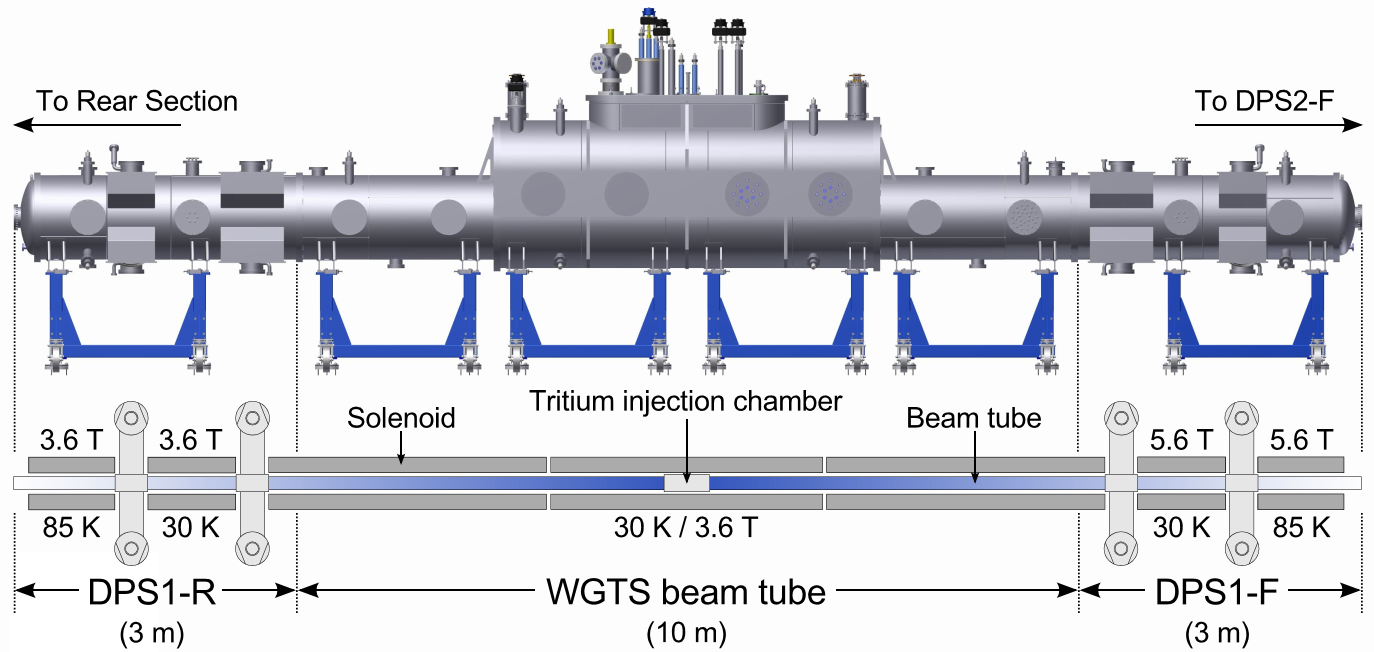
\includegraphics[width=\textwidth]{\currentFigureFolder/wgts.png}
    \xcaption{KATRIN \glsentryfull{wgts}}{The \glsentryfull{wgts}.}{Shown are the hull and a sketch of the beam tube. Indicated are the molecular pumps, the design temperatures for tritium operation, the maximum magnetic field strengths and a color gradient depicting the decreasing gas density from the center to the sides. (From \cite{Harms2015})}
    \label{fig:wgts}
\end{figure}%
The \gls{wgts} is a \SI{16}{m}-long, \SI{1.5}{m}-wide and \SI{4}{m}-high cryostat. It is depicted in figure \ref{fig:wgts} and a detailed description can e.g. be found in \cite{Grohman2008}.
{\par \textbf{The inner loop:} The molecular tritium (\ce{T2}) is injected centrally in the \gls{wgts}'s \SI{90}{mm}-wide beam tube where it decays. The design gas column density is 
\begin{equation}
    \label{eq:columnDensity}
    \rho d = \SI{5e17}{molecules/{cm}^2}
\end{equation}
of which \begin{equation}
    \epsilon_\text{T} = \SI{95}{\percent}
\end{equation}
are isotopic tritium molecules. At the front and rear of the \gls{wgts} the gas is extracted from the beam tube by molecular pumps in designated differential pumping sections called DPS-1-R (rear) and DPS-1-F (front). The extracted gas is re-injected in the center of the beam tube. The respective pipe system is called the inner loop.
\begin{samepage}
Selected important parts of the inner loop are:
\begin{itemize}
\renewcommand{\labelitemi}{$\bullet$}
    \item a buffer vessel where tritium of high purity is introduced from the feed loop of the \gls{tlk};
    \item a \gls{lara} that monitors the isotopic composition of the gas;
    \item a pressure and temperature controlled buffer vessel to regulate the gas inlet into the \gls{wgts}; and
    \item a permeator that separates impurities (like e.g. helium) and ejects them into the exhaust loop of the \gls{tlk}.
\end{itemize}
\end{samepage}}


{\par\textbf{Magnetic field:}
In order to adiabatically guide the $\upbeta$ electrons to the spectrometer section the \gls{wgts} is submerged in a magnetic field parallel to its beam tube of up to \SI{5.6}{T}. It is created by 7 superconducting coils, that surround the beam tube. These magnets are kept at a temperature of \SI{4.2}{K} by liquid helium.}

{\par\textbf{Temperature:}
The stability of the column density \eqref{eq:columnDensity} must be on the \SI{0.1}{\percent} level. This requires stable parameters like temperature $T$ and pressure $p$. On one hand, the higher the temperature the less stable the system. Furthermore, thermal motion smears the energy spectrum of the $\upbeta$ electrons (Doppler effect). On the other hand, at low temperatures the gas molecules cluster. $T=\SI{30}{K}$ is chosen as a compromise and established by a two-phase neon cooling system. For calibration purposes it is also possible to operate the \gls{wgts} with krypton instead of tritium. This requires a beam tube temperature of $T=100K$ in order for the krypton not to freeze. In this operational mode the neon has to be exchanged for argon that provides a suitable vapor pressure.}

\subsection{Rear Section}
\label{sec:rearSection}
\begin{figure}[t]
    \inputpdftex{\currentFigureFolder/rear-section}
   	\xcaption{KATRIN rear section}{The rear section}{terminates the KATRIN beam line and houses several monitoring and calibration devices. (Adapted from \cite{SeitzM2019})}
 \label{fig:rearSection}
\end{figure}

The rear section terminates the beam line in the upstream direction. It houses monitoring, calibration and control devices. It is depicted in figure \ref{fig:rearSection} and a detailed description can e.g. be found in \cite{Babutzka2014}.

{\par \textbf{Rear wall:} The so-called rear wall is a gold-coated stainless-steel disc with a diameter of 6 inches that terminates the beam tube.}

{\par\textbf{Electron gun:}
The rear section houses an electron gun in order to measure the response function of the experiment (see section \ref{sec:response}). Its energy resolution is $\sim \SI{0.2}{eV}$ and its angular resolution is $\sim \SI{4}{\degree}$. The electrons' flight path can be adjusted by dipole magnets mounted in the \gls{wgts} which enables a scanning of the full beam tube.}

{\par\textbf{Plasma control:}
Space charges, respectively a plasma, forms within the \gls{wgts} due to the tritium decay. $\upbeta$ electrons might therefore start at different potentials which adds uncertainty to the measured $\upbeta$ spectrum. Hence, plasma effects have to be controlled. Simulations show that the plasma can be influenced by the rear wall potential which can be controlled by a voltage supply in the range of $\pm \SI{10}{V}$. Moreover, a UV light illumination of the rear wall can extract electrons via the photoelectric effect that can compensate space charges. Details on the plasma in the \gls{wgts} can e.g. be found in \cite{Kuckert2018}.}

{\par\textbf{Activity monitoring:}
$\upbeta$ electrons either arrive at the detector or hit the wall of the experiment. A super conducting coil ensures that the magnetic flux tube terminates at the rear wall. On that account, most $\upbeta$ electrons (\SI{99.99}{\percent}) hit the rear wall where they emit bremsstrahlung. Two dedicated \gls{bixs} systems measure the corresponding X-ray spectrum to determine the source strength respectively the gas column density \eqref{eq:columnDensity}.}

\subsection{Differential Pumping Section}
\label{sec:diffPumpingSection}
\begin{figure}[t]
    \inputpdftex{\currentFigureFolder/dps}
   	\xcaption{KATRIN \glsentryfull{dps}}{The \glsentryfull{dps}}{reduces the gas flow and blocks tritium ions. (Adapted from \cite{SeitzM2019})}
 \label{fig:dps}
\end{figure}
The \glsentryfull{dps} is an approximately \SI{5}{m}-long cryostat. It is depicted in figure \ref{fig:dps} and a detailed description can e.g. be found in \cite{Kosmider2012}. In short, it fulfills the following tasks:

{\par\textbf{Reduction of tritium flow:}
The \glsentryfull{dps} consists of 5 beam tube elements with pump ports between them. The beam tube elements form a \SI{20}{\degree} angle to each other and are arranged in a chicane. While $\upbeta$ electrons are magnetically guided along the chicane, the neutral gas molecules scatter off the walls. This reduces the molecular beaming effect and enhances the pumping probability. Turbo molecular pumps then reduce the gas flow by approximately 5 orders of magnitude and feed the gas into the so-called outer loop where it is reprocessed.}

{\par\textbf{Ion blocking:}
In the \gls{wgts} ions such as \ce{HeT^+}, \ce{T_2+}, \ce{T_3+}, \ce{T_5+} can form. If not blocked, they reach the spectrometer section analogously to the electrons which would eventually lead to an increased background rate. A potential barrier created by two ring electrodes set to $+\SI{100}{V}$ avoids this. The positive ions are deflected, drift out of the flux tube, hit the wall and get neutralized.}

{\par\textbf{Ion monitoring:}
Downstream of the blocking electrodes the remaining ion flux is measured by a Fourier transform ion cyclotron resonance device (FT-ICR). Details on ion forming and their measurement can e.g. be found in \cite{Ubieto2009}.}

\subsection{Cryogenic Pumping Section}
\label{sec:cryoPumpingSection}
\begin{figure}[t]
    \inputpdftex{\currentFigureFolder/cps}
   	\xcaption{KATRIN \glsentryfull{cps}}{The \glsentryfull{cps}}{is the coldest part of the KATRIN experiment. Parts of its beam tube a covered by a frozen argon layer at \SI{3}{K} to cold-trap tritium molecules. The low temperatures are established using liquid helium (\ce{LHe}) and an insulation of liquid nitrogen (\ce{LN2}). (Adapted from \cite{SeitzM2019})}
 \label{fig:cps}
\end{figure}

The \glsentryfull{cps} is an approximately \SI{7}{m}-long cryostat. It is depicted in figure \ref{fig:cps} and a detailed description can e.g. be found in \cite{Jansen2015}. In short, it fulfills the following tasks:
{\par\textbf{Reduction of tritium flow:}
The \gls{cps} consists of 7 beam tube elements of which 5 are arranged in a similar manner as the beam tube elements of the \gls{dps} in a chicane forming \SI{15}{\degree} angles. While charged particles are guided along the chicane by a magnetic field, neutral molecules hit the wall. The walls are covered by a frozen argon layer cooled down to \SI{3}{K} in order to cold-trap particles. After the accumulation of about \SI{1}{Ci} of tritium the argon frost layer has to be renewed. To achieve this the beam tube is warmed-up and the argon is pumped off along with the accumulated tritium. Tests and simulations show a reduction of the tritium flow by approximately 10 orders of magnitude.}

{\par\textbf{The \glsentryfull{fbm}}: The \glsentryshort{fbm} is a detector that can be moved horizontally into the pump port of the \gls{cps} with a 2-dimensional spacial resolution of \SI{0.1}{mm}. Two pin-diodes measure the $\upbeta$ electron flux and hence, the stability of the column density \eqref{eq:columnDensity}. Furthermore, the \gls{fbm} equips a temperature and a hall sensor. A second detector board holding a Faraday cup for ion measurements is also available. Details on the \gls{fbm} can e.g. be found in \cite{Ellinger2017}.}

{\par\textbf{The \glsentryfull{ckrs}} is a sub mono-layer of \kryptonEightyThree{} on a pyrolytic graphite substrate with a diameter of \SI{2}{cm}. It can be lowered in the pump port of the \gls{cps} and moved in a 2-dimensional plane perpendicular to the beam line. This enables the spacial scanning of the properties of the spectrometer using quasi-monoenergetic conversion electron lines of \kryptonEightyThree. Details on the \glsentryshort{ckrs} can e.g. be found in \cite{Bauer2014}.}

\subsection{Pre and Main Spectrometer}
\label{sec:spectrometer}

The pre and main spectrometer are vacuum vessels designed to filter passing electrons according to their kinetic energy. The pre spectrometer has a length of \SI{3.4}{m} and a diameter of \SI{1.7}{m}. Details on its design can e.g. be found in \cite{Prall2012}. The main spectrometer has a length of \SI{23}{m} and a diameter of \SI{10}{m}. Details on its design can e.g. be found in \cite{Angrik:2005ep}.

{\par \textbf{\Gls{mace}}: The pre and main spectrometer apply the so-called \glsentryshort{mace} principle. A retarding voltage deflects electrons with insufficient kinetic energy. The electric field gradient is parallel to the beam line, but $\upbeta$ electrons might be emitted in an arbitrary angle. In order to analyze their full kinetic energy they have to be collimated. This is done by a magnetic field gradient. A quantitative description of this process can be found in section \ref{sec:intSpecModel}. The precision of the \gls{mace} principle increases with the size of the spectrometer. That is why the main spectrometer of KATRIN has a larger diameter (\SI{10}{m}) as the the ones of its predecessor experiments.
}

{\par \textbf{Magnetic field:} The main spectrometer is surrounded by a system of coils that creates the \gls{mace} filter's  magnetic field. Upstream, there is the PS2 magnet; downstream the pinch as well as the detector magnet, which are superconducting solenoids. Their field is fine-tuned by a system of air coils around the spectrometer hull. There is the \gls{emcs} with coils parallel and perpendicular to the beam line axis. Furthermore, there is the \gls{lfcs} with coils perpendicular to the beam line axis. The combined system constrains the electrons' flux tube to the spectrometer vessel and compensates the earth's magnetic field as well as effects from ferromagnetic materials in the spectrometer's surroundings. Details on the magnetic field settings can e.g. be found in \cite{Erhard2018}. Additionally, a vertical and radial magnetic measuring system (\glsentryshort{vmms} and \glsentryshort{rmms}) are installed. The field inside the spectrometer vessel is assessed via samples of these measuring systems combined with simulations. Details on the \glsentryshort{vmms} and the \glsentryshort{rmms} can e.g. be found in \cite{Letnev2018}.}

{\par \textbf{Electric field:} A high voltage system establishes the \gls{mace} filter's retarding potential. According to the KATRIN Design Report \cite{Angrik:2005ep} the retarding voltage's fluctuations must have a standard deviation smaller than \SI{60}{mV} for the envisaged sensitivity on the neutrino mass. The antenna-like beam line setup is sensitive to electromagnetic fluctuations, which is why an active so-called post-regulation system is deployed. It monitors the retarding potential and regulates it with the needed precision. For the monitoring exist the so-called monitor spectrometer and a voltage divider. Details on the voltage calibration with the voltage divider can e.g. be found in \cite{Thuemmler2009}. The monitor spectrometer is part of a second beam line in a separate building. Its retarding potential follows the one one of the main spectrometer and is measured via \kryptonEightyThree{} conversion lines. Details on the monitor spectrometer can be e.g. be found in \cite{Erhard2014}.}

{\par \textbf{Background:} According to the KATRIN Design Report \cite{Angrik:2005ep} the electron rate of uncontrollable sources (background) must be less than \SI{10}{mHz}. Several background-related aspects are:}

{\par \textbf{Vacuum:} The spectrometers are operated at a pressure on the order of \SIrange{10e-11}{10e-12}{mbar}. This prevents electron scattering on residual gas and minimizes background effects by ionization. Correspondingly, several turbo molecular and getter pumps are installed at the spectrometer vessels. Furthermore, the spectrometers can be baked out at up to \SI{350}{\celsius}. Details on the vacuum system can e.g. be found in \cite{Arenz2016}.}

{\par \textbf{Wire electrodes:} The inner walls of the spectrometer vessels are lined by wire electrodes. Their potential is at a few hundred volts below the spectrometer hull reflecting electrons coming from the vessel walls. These electrons might be induced by e.g. cosmic rays or emanate from the spectrometer wall. A detailed description of the wire electrodes can e.g. be found in \cite{Valerius2009}.}

{\par \textbf{Ion blocking:} Analogously to the ones in the \gls{cps} (section \ref{sec:cryoPumpingSection}), three blocking electrodes are installed; one between the \gls{cps} and the pre spectrometer, one between the pre and main spectrometer; and one between the main spectrometer and the detector.}

{\par \textbf{Tandem setup:} $\upbeta$ electrons might scatter on residual gas or the beam line walls. This can either directly lead to secondary electrons or create positive ions that travel down the beam line. The positive ions in turn might again through scattering yield secondary electrons. The more $\upbeta$ electrons enter the main spectrometer the higher is the probability to create secondary electrons. In order to reduce the flux of $\upbeta$ electrons into the main spectrometer the retarding potential of the pre spectrometer is set to a few hundred volts below the one of the main spectrometer. On one hand this is a countermeasure against background events. But on the other hand, charged particles can be trapped between the two spectrometers due to the electromagnetic setup (Penning trap). A sudden discharge might harm the hardware, especially the detector. Therefore, it is possible to sweep a charged wire through the volume in order to collect the trapped particles and avoid this ``Penning-discharges''.}

\subsection{Detector Section}
\label{sec:detector}
\begin{figure}[t]
    \inputpdftex{\currentFigureFolder/detector-section}
   	\xcaption{KATRIN detector section}{The detector section}{terminates the KATRIN beam line. Among other instruments it houses the \glsentrylong{fpd} for $\upbeta$ electrons with the detector wafer at its core.(Adapted from \cite{SeitzM2019})}
 \label{fig:detector}
\end{figure}

The detector section terminates the beam line in downstream direction. It can be separated from the spectrometer section by closing a gate valve. The detector section is depicted in figure \ref{fig:detector} and a detailed description can e.g. be found in \cite{Amsbaugh2015}.

{\par \textbf{The \gls{fpd}} counts the $\upbeta$ electrons that pass the spectrometer section. The \gls{fpd} is a pin-silicon detector with a sensitive area of \SI{9}{cm} diameter. It is subdivided in 148 pixels of the same area arranged in 12 rings of 12 pixels each and the so called bull's eye of 4 pixels in the center. This arrangement allows later correction for radial electrical and magnetic inhomogeneities in the beam line.}

{\par \textbf{Shield and veto system:} The \gls{fpd} system's radiation shield consists of two nested cylindrical shells: an outer lead shell of \SI{3}{cm} that reduces photon background and an inner copper shell of \SI{1.27}{cm} that blocks X-rays originating from the outer lead shell. The shield is surrounded by a veto system to tag incoming muons.}

{\par \textbf{Calibration:} Photoelectron sources can be lowered in the detectors line of sight. The corresponding photocurrent can be measured with the so-called \gls{pulcinella} system. A comparison of \gls{pulcinella} and the \gls{fpd} yields the \gls{fpd}'s detection efficiency.}

{\par \textbf{The detector magnet} allows to form the flux tube near the detector independently of the main spectrometer magnetic field setting. This is especially useful in the above mentioned calibration process.}

{\par \textbf{The post-acceleration electrode} allows to shift the energy of $\upbeta$ electrons arriving from the main spectrometer. This way $\upbeta$ electrons can be distinguished from background electrons originating in the detector section by an energy region of interest cut.}